% Capitulo 3 - Análise de Sinais
\chapter{\captres}\label{analise}
\par
Para a proteção dos \ac{SEP}, foram criados vários métodos para diagnóstico de faltas em linhas de transmissão. Estes métodos podem ser divididos em métodos convencionais, métodos baseados em análise de sinais e métodos baseados em sistemas inteligentes.
\par
Os métodos convencionais utilizam uma variedade de parâmetros para tomada de decisão sobre a ocorrência da falta, sendo que os parâmetros mais comuns são a tensão e a corrente da linha. 
\par
Os métodos baseados em sistemas inteligentes utilizam dados extraídos da linha como padrões de entrada para o sistema inteligente, tais como \ac{RNAs}, \emph{Lógica Fuzzy} ou \emph{Redes Neurofuzzy} \cite{INA10}. 
\par 
Já os métodos baseados em análise de sinais utilizam os transitórios de alta frequência gerados pela falta na linha para sua detecção, onde os transitórios são extraídos dos sinais de tensão ou corrente, empregando ferramentas matemáticas. 
\par
Aborda-se neste capitulo especialmente esses três métodos, \emph{\ac{RMS}},\emph{\ac{TF}} e \emph{\ac{TW}}, assim como conceitos sobre amostragem de dados, filtros e decomposição de sinais.
\section{Amostragem de dados}
\par
Definido por \cite{SIL09}, na realização da maioria dos estudos estatísticos, não é possível ou conveniente levantar os dados de todos os elementos da população. Nesses casos, é estudada uma amostra proveniente da população e buscada, através da estatística indutiva, para tirar conclusões sobre a população.
\par
O processo usado para selecionar a amostra (amostragem) deve ser usado com bastante cuidado, uma vez que, se for equivocado no momento de selecionar os elementos da amostra, os resultados finais podem ser incorretos \cite{SIL09}. 
\par Colocado por \cite{SIL09}, existem diversos tipos de amostragem, que, em geral são classificados em probabilísticos e não probabilísticos, respectivamente, de forma simplificada são os processos de escolha da amostra de forma aleatória ou não aleatória.
De acordo com \cite{BAC11}, a amostragem de dados é importante para a realização da análise de tensão elétrica, para a realização da detecção e identificação dos distúrbios eletromagnéticos, para tanto, se faz necessário à utilização de técnicas de \ac{DSP}.
\par
O uso dos equipamentos industriais, em geral, tem sua utilização variável ao longo do dia, da semana e/ou do mês. Deve-se determinar o tamanho da menor amostra capaz de representar o comportamento do equipamento ao longo do período da fatura de energia elétrica \cite{BAC11}.
\section{Métodos baseados em análise de sinais}
\par
De acordo com \cite{JUN09}, o gerenciamento dos fenômenos eletromagnéticos associados à \ac{QEE} iniciaram-se nas décadas de 70 e 80 com o surgimento de osciloscópios e sistemas de visualizações gráficas.
\par
As técnicas aplicadas atualmente somente tiveram sua utilização em larga escala a partir da década de 90. Este fato deve-se aos avanços obtidos na área de processamento de sinais, a redução dos custos dos sistemas de monitoração e ao aprofundamento do conhecimento sobre aplicações de processamentos de sinais em sistemas potência.
\par
Tais acontecimentos impactaram com grande relevância para a utilização destas técnicas na monitoração da \ac{QEE}. Os principais métodos utilizados para detectar os fenômenos eletromagnéticos são:
\begin{itemize}
\item Método baseado no cálculo do Valor \ac{RMS}; 
\item Método baseado na aplicação da Transformada Discreta de Fourier;
\item Método baseado na aplicação da Transformada Wavelet.
\end{itemize}
\subsection{Método baseado no cálculo do Valor \ac{RMS}}
\par
O valor eficaz ou RMS é uma das técnicas mais utilizadas para a detecção de eventos que afetam \ac{QEE} \citep{KAG09}
, citado por \citep{BAC11}. Segundo \cite{THE99}, citado por \cite{JUN09}, esta técnica consiste na monitoração dos valores de tensão \ac{RMS} em tempo real do sistema com a finalidade de detectar os distúrbios. A detecção de eventos pode ser realizada através da comparação do valor \ac{RMS} da tensão com uma faixa de tolerância. 
\par 
O calculo do valor \ac{RMS} do sinal monitorado é realizado \emph{através de janelas de 1 ou 1/2 ciclo da componente fundamental}, essas janelas são pré-determinadas, são caracterizadas por \emph{n} amostras por \emph{m} pontos por amostranges, definindo o seu deslocamento de dados durante a amostragem. 
\todo[inline,color=red]{Fazer. Para maiores informações sobre RMS consultar bli em blo e blu.}
\subsection{Método baseado na aplicação da Transformada Discreta de Fourier}
\par
A \acl{TF} pode ser considerada como a soma de funções trigonométricas (\emph{senoidal} e\emph{ cossenoidal}) ou de exponenciais complexas harmonicamente relacionadas \citep{KAG09}, citado por \citep{BAC11}.
\par
De acordo com \cite{SAD03}, a \ac{SF} permite representar uma função periódica como a soma de senoides obtendo o espectro de frequência da série. A \ac{TF} nos permite estender o conceito de espectro de frequência a funções não periódicas. A transformada considera que uma função não periódica é uma função periódica com período infinito. Por tanto, a \ac{TF} é uma representação integral de uma função não periódica, análoga à representação em \ac{SF} de uma função periódica.
\par
A \acl{TF} é uma \emph{Transformada Integral}, como a \emph{Transformada de Laplace}, esta transforma uma função do domínio de tempo para o domínio de frequência. Esta transformada é muito útil em sistemas de comunicação e no uso de \ac{DSP}, situações nas quais geralmente a \emph{Transformada de Laplace} não se aplica. A \ac{TF} pode trabalhar com circuitos tanto com entradas para \emph{t < 0} quando para \emph{t > 0}, \citep{SAD03}.
\todo[inline,color=red]{Fazer. Para maiores informações sobre TF E sua familia, consultar bli em blo e blu.}
\par
Segundo \cite{OLI07}, a \ac{TF} tem suas grandes vantagens, porém possui uma grande desvantagem. Embora esta possa determinar todas as frequências presentes no sinal, sua relação com o domínio temporal é inexistente, a \ac{TF} é não fornece uma análise temporal, \emph{apenas frequencial}.
\par
Complementando este esclarecimento sobre a desvantagem descrita anteriormente, \cite{MEN08} esclarece que se as propriedades de um sinal não variarem muito ao longo do tempo, ou seja, se o sinal for estacionário, esta desvantagem não é muito importante. No entanto, grande parte dos sinais contêm inúmeras características transitórias ou não estacionárias e estas características podem ser a parte mais importante do sinal, então a transformada de Fourier não é apropriada à sua detecção. 
\par
Para superar esse problema, várias alternativas foram propostas objetivando ter uma análise, ao mesmo tempo, temporal e frequencial de sinais não estacionários. A primeira dessas alternativas foi a \ac{STFT}, também conhecida como a Transformada de Gabor \citep{OLI07}.
\par 
Explicado por \cite{OLI07}, o objetivo da STFT é introduzir um parâmetro de frequência local (local ao tempo) como se a Transformada de Fourier Local observasse o sinal através de uma curta janela (técnica de janelamento) dentro da qual o sinal permanece aproximadamente estacionário, exemplificada na Figura \ref{fig:janelamento}.
% figura 2
\begin{figure}[!h]
\begin{center}
\caption{Análise local no tempo: o uso de janelas.}
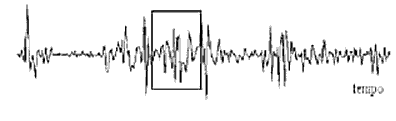
\includegraphics[height=3cm]{imagens/janelamento.png}
\par{\small Fonte: Extraída de \cite{OLI07}.}
\label{fig:janelamento}
\end{center}
\end{figure}
\par
A \ac{STFT} fornece informações sobre quando e a que frequências um determinado evento ocorrente no sinal. No entanto, essa informação só pode ser obtida com determinada precisão, e essa precisão é limitada pelo tamanho da janela, causando outra desvantagem nesta técnica, cujo tamanho fixo dessa janela deslizante não pode ser alterada ao longo na análise, necessitando ser a mesma para todas as frequências. 
\par
Muitos sinais (especialmente no caso de detecção de distúrbios elétricos) requerem uma técnica mais flexível, onde seja possível variar o tamanho da janela para determinar com melhor precisão na base tempo ou na base frequência,\citep{MEN08}.
\subsection{Método baseado na aplicação da \acl{TW}}
\par
Em %\cite{KIM01} 
e \cite{IAN09} citados por \cite{FER10}, a \acl{TW} vem sendo extensivamente aplicada à análise de distúrbios elétricos. A frequente utilização da \ac{TW} se dá pela sua habilidade de destacar curtos transitórios em componentes de alta frequência e longos transitórios em componentes de baixa frequência, tal habilidade facilita a análise de impulsos e transitórios localizados mesmo na presença do componente fundamental e harmônicos de baixa ordem. 
\par
Explicitado por \cite{OLI07}, as \emph{Wavelets} são funções matemáticas que separam dados em suas diferentes componentes frequências e extraem cada componente com uma resolução adequada à sua escala. Elas têm vantagens em relação à análise de \textit{Fourier}, pois esta última analisa o sinal como um todo, acarretando uma representação mais pobre para sinais que contêm descontinuidades e variações bruscas.
\par
Segundo \cite{MEN08}, \cite{OLI07} e \cite{FER10}, a \ac{TW} também faz uso de uma janela deslizante que se adapta automaticamente com regiões de tamanhos variáveis, de acordo com as frequências presentes no sinal em análise, gerando uma resolução apropriada em componentes de altas e baixas frequências. A acl{TW} possui suas variantes contínua (TWC) e discreta (TWD) para maiores detalhes sobre as definições matemáticas das TWC e TWD consulte o Anexo G em \cite{FER10} ou no capítulo dois e três, respectivamente, em \citep{OLI07}. 
\par
No trabalho de \cite{MEN08}, é feita uma comparação com a \textit{base-tempo}, \textit{base-frequência} e com a \ac{STFT}, explicitas na Figura \ref{fig:analisis}. É possível observar que as \textit{Wavelets} não utilizam uma região \emph{tempo-frequência}, mas sim uma região \emph{tempo-escala}.
% figura 3
\begin{figure}[!h]
\begin{center}
\caption{Comparação de bases entre Análise de Fourier e Análise de Wavelet.}
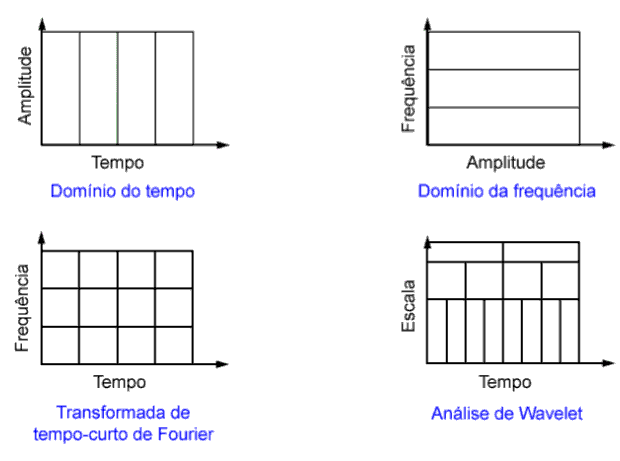
\includegraphics[height=8cm]{imagens/cap3_analisis.png}
\par{\small Fonte: Extraída do trabalho de \cite{MEN08}.}
\label{fig:analisis}
\end{center}
\end{figure}
\subsection{Filtragem e decomposição de sinais}
\par
As componentes dos sinais fornecem características tipicas de acordo com as frequências utilizadas, componentes de baixa frequência fornecem a identidade do sinal e as componentes de alta frequência, por outro lado, fornecem os detalhes do sinal. Um exemplo disto é a análise da voz humana. Se retirarmos as componentes de alta frequência, a voz terá um som diferente, mas é possível entender o que está sendo dito.
\par
No entanto, se retirarmos as componentes de baixa frequência, será emitido um palavreado sem sentido \cite{MIS96}, citado por \cite{DEL03}. Por esta razão que, em análise Wavelet, fala-se usualmente em aproximações e detalhes.
\par
As aproximações são as componentes de baixa frequência do sinal e os detalhes são as componentes de alta frequência do sinal. O processo de filtragem, em seu nível mais básico, é mostrado na Figura \ref{fig:filtragem}. O sinal \textbf{S} percorre dois filtros complementares que fornecem dois sinais como saída. Porém, se utilizarmos este esquema em um sinal digital real, obtém-se duas vezes mais a quantidade de dados que no início, podendo-se incluir técnicas de redução da amostragem para não ter uma superpopulação de dados após esse processo de filtragem. 
\par 
Decomposição do sinal, conforme \cite{JUN09}, citado por \cite{BAC11}, é uma forma de detecção de perturbações em um sistema estável de 60 Hz é a decomposição do sinal em sua componente fundamental de (60 Hz) e em uma componente residual contendo os demais componentes. O sinal adquirido pelo sistema de amostragem de dados deve ser digitalizado e depois de decomposto para que possa ser utilizado por algum sistema computacional.
% figura 4
\begin{figure}[!h]
\begin{center}
\caption{Processo de filtragem ao nível mais básico.}
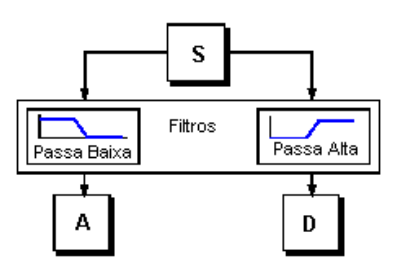
\includegraphics[height=5cm]{imagens/figura-filtragem.png}
\par{\small Fonte: Figura retirada de \cite{MEN08}.}
\label{fig:filtragem}
\end{center}
\end{figure}
\par
A Decomposição de nível múltiplo é um processo de decomposição que pode ser \emph{iterado}, com sucessivas aproximações a serem decompostas, de forma que um sinal seja dividido em muitas componentes de baixa resolução. Isto é chamado de \emph{árvore de decomposição de Wavelet} \citep{MEN08}, demonstrada na Figura \ref{fig:decomp}.
% figura 5
\begin{figure}[!h]
\begin{center}
\caption{Árvore de decomposição de Wavelet}
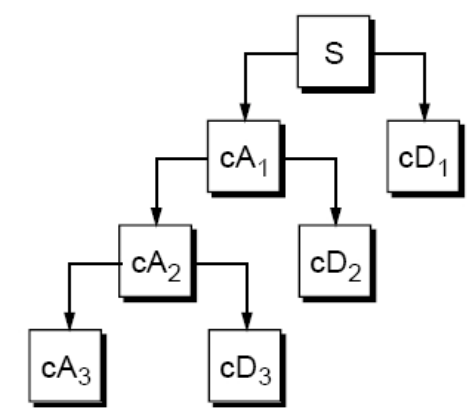
\includegraphics[height=8cm]{imagens/figura-decmult.png}
\par{\small Fonte: Figura capturada no trabalho de \cite{MEN08}.}
\label{fig:decomp}
\end{center}
\end{figure}
\par
No trabalho de \cite{BAC11}, é demonstrado a partir da simulação de um transitório oscilatório (produzido pelo chaveamento de um capacitor), onde é utilizado como exemplo para aplicação de uma série de decomposições de \ac{TW}. Observando à Figura \ref{fig:decomptw}(a) o primeiro nível de decomposição e na Figura \ref{fig:decomptw}(b) os coeficientes de detalhes, que demonstram de forma clara a ocorrência do evento oscilatório.
% figura 6
\begin{figure}[!h]
\begin{center}
\caption{Decomposição de sinais utilizando \ac{TW}}
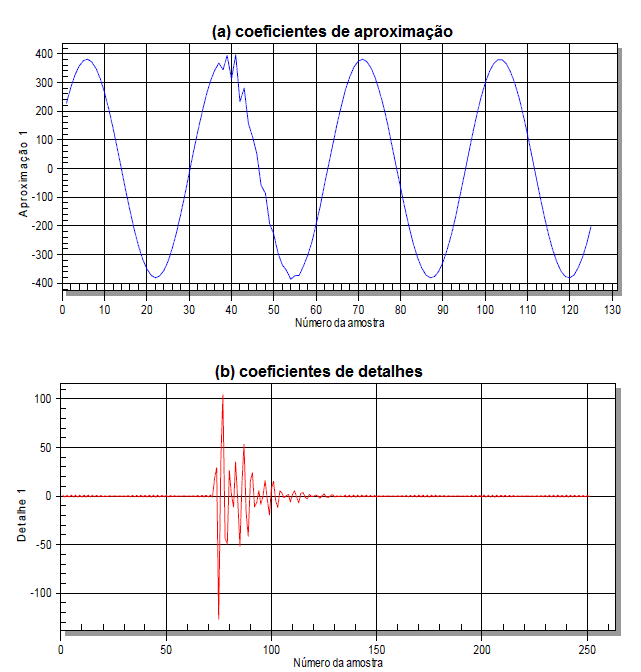
\includegraphics[height=8cm]{imagens/decompsinais.png}
\par{\small Fonte: Figura fornecida por \cite{BAC11}.}
\label{fig:decomptw}
\end{center}
\end{figure}
\par
A análise de sinais, dentro do trabalho proposto, possui papel fundamental para a identificação dos distúrbios elétricos, definidos e explanados no capitulo anterior. O uso desta importante ferramenta permite a realização da analise dos dados de amostragem, e no qual em sua falta não poderia ser feita para extração dos parâmetros de \ac{QEE}. O da análise de sinais é interno do sistema computacional proposto, e integra tanto o sistema embarcado envolvido quanto a simulação do sistema, ambas as definições estão dispostas no próximo capítulo \ref{Estruturas}.